\documentclass[11pt,a4paper]{article}
\usepackage[margin=25mm,headheight=15pt]{geometry}
\usepackage[T1]{fontenc}
\usepackage[utf8]{inputenc}
\usepackage{amsmath,amsthm,mathtools}
\usepackage{newpxtext,newpxmath}
\usepackage{microtype}
\usepackage{booktabs,array,graphicx,float,placeins}
\usepackage{xcolor}
\usepackage[most]{tcolorbox}
\usepackage{enumitem}
\usepackage{xurl}
\usepackage{hyperref}
\usepackage{fancyhdr}
\usepackage{listings}
\definecolor{ink}{HTML}{15334A}
\definecolor{soft}{HTML}{F3F6F8}
\definecolor{muted}{HTML}{536572}
\hypersetup{colorlinks=true,linkcolor=ink,citecolor=ink,urlcolor=ink,
 pdftitle={Asymptotics of OEIS A277364},
 pdfauthor={Mathematical analysis prepared with ChatGPT},
 pdfsubject={Bell numbers, truncated Stirling sums, saddle-point asymptotics}}
\pagestyle{fancy}
\fancyhf{}
\fancyhead[L]{\small\textsc{Asymptotics of OEIS A277364}}
\fancyhead[R]{\small Bell growth and the omitted tail}
\fancyfoot[C]{\thepage}
\renewcommand{\headrulewidth}{0.35pt}
\setlength{\parindent}{1.1em}
\setlength{\parskip}{3pt}
\setlength{\emergencystretch}{2em}
\allowdisplaybreaks[2]
\numberwithin{equation}{section}
\newtheorem{theorem}{Theorem}[section]
\newtheorem{lemma}[theorem]{Lemma}
\newtheorem{proposition}[theorem]{Proposition}
\newtheorem{corollary}[theorem]{Corollary}
\theoremstyle{remark}
\newtheorem{remark}[theorem]{Remark}
\newcommand{\e}{\mathrm e}
\newcommand{\ii}{\mathrm i}
\newcommand{\Prob}{\mathbb P}
\newcommand{\Expect}{\mathbb E}
\newcommand{\Var}{\operatorname{Var}}
\newcommand{\coef}[2]{[#1^{#2}]}
\newcommand{\Stir}[2]{\left\{\begin{matrix}#1\\#2\end{matrix}\right\}}
\newcommand{\bigO}{\mathcal O}
\newtcolorbox{resultbox}{colback=soft,colframe=ink,boxrule=.6pt,
 arc=1mm,left=10pt,right=10pt,top=8pt,bottom=8pt,breakable}
\lstset{basicstyle=\ttfamily\small,breaklines=true,columns=fullflexible,
 frame=single,rulecolor=\color{muted},showstringspaces=false}

\title{\color{ink}\bfseries Asymptotics of OEIS A277364\\[5pt]
\large Bell-number growth and a parity-sensitive omitted tail}
\author{A mathematical analysis prepared for Vladimir Reshetnikov}
\date{20 September 2026}

\begin{document}
\maketitle
\begin{abstract}
The sequence A277364 counts partitions of an $n$-element set into at most
$\lfloor n/2\rfloor$ nonempty blocks. We prove that this restriction removes an
asymptotically negligible proportion of all set partitions, and hence that the
sequence has the full Bell-number asymptotic expansion at every algebraic
relative-error scale. Writing $r=W_0(n)$, its leading equivalent is
\[
 a(n)\sim\frac{\exp\{n(r-1+r^{-1})-1\}}{\sqrt{1+r}}.
\]
We give a self-contained saddle-point proof, the explicit first correction,
and an elementary proof that truncation is harmless. We also determine the
much smaller difference $B_n-a(n)$: it is asymptotic to the first omitted
Stirling number and has a parity-dependent prefactor multiplying
$(C\sqrt n)^n$, where $C=1.0658863584\ldots$. The omitted proportion is
$\exp\{-\tfrac12n\log n+n\log\log n+O(n)\}$.
An explicit first correction for this tail, a fixed-fraction generalization,
and reproducible exact-integer computations complete the analysis.
\end{abstract}

\section{Definition and principal conclusions}

The OEIS entry defines A277364 by the finite Stirling sum
\begin{equation}\label{eq:def}
 a(n)=\sum_{k=0}^{\lfloor n/2\rfloor}S(n,k),
 \qquad S(n,k)=\Stir nk.
\end{equation}
The entry was contributed by Vladimir Reshetnikov in 2016. Its displayed
terms begin
\[
1,0,1,1,8,16,122,365,2795,11051,86472,422005,\ldots.
\]
The definition and these initial values are taken from the retrieved OEIS
entry~\cite{oeis}; the calculations below independently reproduce all 26
values displayed there. In particular, $a(0)=1$ and $a(1)=0$.

Let
\begin{equation}\label{eq:taildef}
 B_n=\sum_{k=0}^nS(n,k),\qquad
 K_n=\lfloor n/2\rfloor+1,\qquad
 D_n=B_n-a(n)=\sum_{k=K_n}^n S(n,k).
\end{equation}
Thus $B_n$ is the $n$th Bell number. Our convention is that the blocks are
nonempty and unordered, and the elements are labeled, as in the standard
Bell and Stirling definitions~\cite{dlmf-bell,dlmf-stirling}.

\begin{remark}[What is, and is not, being restricted]
The bound concerns the \emph{number of blocks}, not their individual sizes.
Singleton blocks are allowed. For example,
$\{\{1\},\{2,3,4\}\}$ is counted when $n=4$.
The condition says that the average block size is at least two, not that
every block has size at least two.
\end{remark}

Throughout the article, logarithms are natural unless a base is specified.
The notation $f(n)\sim g(n)$ means that $f(n)/g(n)\to1$.
Let $W_0$ denote the principal real Lambert function, so that
\begin{equation}\label{eq:W}
 r=r_n=W_0(n)>0,\qquad r\e^r=n.
\end{equation}
Define
\begin{align}
 F(n)&=\frac{\exp\{n(r-1+r^{-1})-1\}}{\sqrt{1+r}},\label{eq:F}\\
 P(r)&=\frac{r^2(2r^2+7r+10)}{24(1+r)^3}.\label{eq:P}
\end{align}

\begin{theorem}[Asymptotic growth]\label{thm:main}
As $n\to\infty$,
\begin{equation}\label{eq:main}
 a(n)=F(n)\left(1-\frac{P(r)}n+
 O\!\left(\frac{r^2}{n^2}\right)\right).
\end{equation}
In particular,
\begin{equation}\label{eq:equivalent}
 \boxed{\displaystyle
 a(n)\sim B_n\sim
 \frac{1}{\sqrt{1+W_0(n)}}
 \left(\frac{n}{\e W_0(n)}\right)^n
 \exp\!\left(\frac{n}{W_0(n)}-1\right).}
\end{equation}
Consequently, on the coarser logarithmic and root scales,
\begin{align}
 \log a(n)&=n\log n-n\log\log n-n+o(n),\label{eq:logcoarse}\\
 a(n)^{1/n}&\sim\frac{n}{\e\log n}.\label{eq:root}
\end{align}
\end{theorem}

The Bell-number factor in this theorem is classical. Moser and Wyman
obtained a full saddle-point expansion~\cite{moser-wyman}; NIST records the
leading equivalent in terms of the solution of $N\log N=n$~\cite{dlmf-bell}.
The task particular to A277364 is to justify discarding the upper half of
the Stirling row. We prove this first without using any Bell asymptotic.
We subsequently quantify the discarded part itself.

\begin{resultbox}
\textbf{Growth-rate summary.}
A277364 has Bell-number growth, not the much smaller growth of the
boundary term $S(n,\lfloor n/2\rfloor)$. The number of summands alone is
misleading: the substantial mass of the Stirling row lies well to the left
of the cutoff. The omitted fraction satisfies
\[
 \log\frac{B_n-a(n)}{B_n}
 =-\frac12n\log n+n\log\log n+O(n).
\]
In particular, it is smaller than $\e^{-cn}$ for every fixed $c>0$, once
$n$ is sufficiently large.
\end{resultbox}

\section{An elementary proof that the cutoff is negligible}

\begin{lemma}[Two elementary counting bounds]\label{lem:counting}
For $1\le k\le n$,
\begin{equation}\label{eq:countbounds}
 k^{n-k}\le S(n,k)\le\binom nk k^{n-k}.
\end{equation}
Consequently,
\begin{equation}\label{eq:crudeD}
 D_n\le 2^n n^{n-K_n}\le 2^n n^{n/2}.
\end{equation}
\end{lemma}
\begin{proof}
For the lower bound, place elements $1,\ldots,k$ in distinct blocks and
assign each of the remaining $n-k$ elements to one of those blocks. The
resulting partitions are distinct, giving $k^{n-k}$ possibilities.

For the upper bound, encode a partition by its set of $k$ block minima and,
for every other element, the minimum of its block. There are at most
$\binom nk k^{n-k}$ such encodings. Some encodings do not correspond to a
valid set of minima, which only makes the upper bound more generous.
For $k\ge K_n$, we have $k^{n-k}\le n^{n-K_n}$. Summing over these $k$ and
using $\sum_k\binom nk=2^n$ gives~\eqref{eq:crudeD}.
\end{proof}

\begin{proposition}[Super-exponentially small omitted proportion]
\label{prop:negligible}
There is a constant $C_0$ such that, for all sufficiently large $n$,
\begin{equation}\label{eq:elementaryratio}
 0<\frac{D_n}{B_n}
 \le\exp\!\left(-\frac12n\log n+n\log\log n+C_0n\right).
\end{equation}
Hence $a(n)/B_n\to1$, and $D_n/B_n=o(n^{-M})$ for every fixed $M>0$.
\end{proposition}
\begin{proof}
Take $k=\lfloor n/\log n\rfloor$. The lower bound in
Lemma~\ref{lem:counting} gives $B_n\ge k^{n-k}$. Since
\[
 \log k=\log n-\log\log n+O(\log n/n),
\]
we have
\begin{equation}\label{eq:lowerlog}
 \log B_n\ge (n-k)\log k
 =n\log n-n\log\log n-n
   +O\!\left(\frac{n\log\log n}{\log n}\right).
\end{equation}
Subtract this lower bound from the logarithm of~\eqref{eq:crudeD}.
The result is~\eqref{eq:elementaryratio} after increasing $C_0$.
Its exponent tends to $-\infty$ faster in magnitude than either $cn$ or
$M\log n$, for any fixed positive $c,M$.
\end{proof}

This proof uses no concentration theorem and no asymptotic formula for
Stirling numbers. It also explains why every fixed-order relative
expansion of $B_n$ in inverse powers of $n$, with logarithmic factors,
transfers unchanged to $a(n)$. The difference is smaller than all such
error scales. An asymptotic expansion of $a(n)$ alone therefore conceals
the interesting parity effect in $D_n$.

\section{The Bell saddle and its first correction}\label{sec:bell}

We now derive the Bell estimate needed for Theorem~\ref{thm:main}.
The generating-function identities
\begin{equation}\label{eq:egfs}
 S(n,k)=\frac{n!}{k!}\coef zn(\e^z-1)^k,
 \qquad
 \sum_{n\ge0}B_n\frac{z^n}{n!}=\exp(\e^z-1)
\end{equation}
follow by forming a set of nonempty labeled blocks. They are also recorded
in NIST's Bell and Stirling sections~\cite{dlmf-bell,dlmf-stirling}.

\subsection{The saddle-point integral}
Cauchy's formula on the circle $z=r\e^{\ii\theta}$ gives
\begin{equation}\label{eq:bellintegral}
 B_n=\frac{n!\exp(\e^r-1)}{2\pi r^n}
 \int_{-\pi}^{\pi}\exp H(\theta)\,d\theta,
 \quad
 H(\theta)=\e^{r\e^{\ii\theta}}-\e^r-\ii n\theta.
\end{equation}
The linear term disappears precisely when $r\e^r=n$.
With $D=z\,d/dz$, the higher angular derivatives are determined by
$D^j\e^z$. In particular, putting
\begin{align}
 b&=n(1+r),\label{eq:bcdb}\\
 c&=n(1+3r+r^2),\\
 d&=n(1+7r+6r^2+r^3),\label{eq:bcdd}
\end{align}
we obtain locally
\begin{equation}\label{eq:hexpand}
 H(\theta)=-\frac b2\theta^2-\frac{\ii c}{6}\theta^3
 +\frac d{24}\theta^4+\cdots.
\end{equation}
The Gaussian width is $b^{-1/2}\asymp(nr)^{-1/2}$.

\subsection{Why the rest of the contour is negligible}
Here are explicit estimates that justify using the local expansion.
The real loss in the exponent is
\begin{equation}\label{eq:loss}
 -\Re H(\theta)
 =\e^r-\e^{r\cos\theta}\cos(r\sin\theta).
\end{equation}
For $|\theta|\le1/r$, elementary sine and cosine inequalities give
\begin{equation}\label{eq:centralbound}
 -\Re H(\theta)\ge c_1nr\theta^2
\end{equation}
with an absolute $c_1>0$, for all sufficiently large $r$. Indeed, the term
$\e^{r\cos\theta}(1-\cos(r\sin\theta))$ alone has this lower bound.
For $1/r\le|\theta|\le\pi$, discard the cosine factor to obtain
\begin{align}
 -\Re H(\theta)
 &\ge\e^r-\e^{r\cos\theta}\notag\\
 &\ge\e^r\bigl(1-\exp\{-r(1-\cos(1/r))\}\bigr)
 \ge c_2 n/r^2.\label{eq:outerbound}
\end{align}
Thus no second part of the circle contributes on the Gaussian scale.

For completeness, set $\varepsilon=\sqrt{r/n}$ and $u=\sqrt b\,\theta$.
For each fixed $j\ge3$,
\begin{equation}\label{eq:standardized}
 \frac{D^j\e^r}{b^{j/2}}=O(\varepsilon^{j-2}).
\end{equation}
This follows from $D^j\e^r=\e^r T_j(r)$, where $T_j$ is a degree-$j$
polynomial. On $|u|\le\varepsilon^{-1/12}$, Taylor expansion of the
exponential, with the Gaussian factor kept outside, has an integrable
polynomial remainder of order $O(\varepsilon^4)$. The terms of orders
$\varepsilon$ and $\varepsilon^3$ are odd and imaginary; they integrate to
zero over this symmetric interval. Estimate~\eqref{eq:centralbound}
handles the remaining interval up to $1/r$, with loss at least a positive
multiple of $\varepsilon^{-1/6}$, and~\eqref{eq:outerbound} handles the
outer arc. Both errors are smaller than any fixed power of $\varepsilon$.
These observations justify the error term in the next calculation, not
merely its formal coefficients.

\subsection{Gaussian contractions}
The first nonzero correction comes from the quartic term and the square
of the cubic term. Since the second, fourth, and sixth centered Gaussian
moments with unit variance are $1,3,15$, respectively,
\begin{equation}\label{eq:bellcoefficient}
 B_n=\frac{n!\exp(n/r-1)}{r^n\sqrt{2\pi n(1+r)}}
 \left(1+\frac d{8b^2}-\frac{5c^2}{24b^3}
       +O\!\left(\frac{r^2}{n^2}\right)\right).
\end{equation}
Substitution of~\eqref{eq:bcdb}--\eqref{eq:bcdd} simplifies the correction to
\begin{equation}\label{eq:precorrection}
 \frac d{8b^2}-\frac{5c^2}{24b^3}
 =-\frac{2r^4+9r^3+16r^2+6r+2}{24n(1+r)^3}.
\end{equation}
Finally,
\[
 n!=\sqrt{2\pi n}(n/\e)^n
       \left(1+\frac1{12n}+O(n^{-2})\right).
\]
The $1/(12n)$ term must be included: it changes the correction from
\eqref{eq:precorrection} to $-P(r)/n$. Using $n/r=\e^r$ gives
\begin{equation}\label{eq:bellfinal}
 B_n=F(n)\left(1-\frac{P(r)}n+O(r^2/n^2)\right).
\end{equation}
Proposition~\ref{prop:negligible} now proves~\eqref{eq:main}.

\begin{remark}[Two normalizations]
Formula~\eqref{eq:bellcoefficient} leaves $n!$ exact, whereas
\eqref{eq:bellfinal} expands it. Their leading terms are equivalent, but
their first correction coefficients differ by $1/12$. Mixing the
prefactor from one normalization with the correction from the other
produces an incorrect first-order formula.
\end{remark}

\section{Logarithmic growth, ratios, and interpretation}\label{sec:consequences}

\subsection{A logarithmic expansion}
Taking logarithms in~\eqref{eq:main} yields the comparatively precise form
\begin{equation}\label{eq:logprecise}
 \log a(n)=n(r-1+r^{-1})-1-\frac12\log(1+r)
          -\frac{P(r)}n+O(r^2/n^2).
\end{equation}
Let $L=\log n$ and $\ell=\log\log n$. The expansion obtained by solving
$r+\log r=L$ is
\begin{equation}\label{eq:Wexpand}
 r=L-\ell+\frac\ell L+\frac{\ell(\ell-2)}{2L^2}
   +\frac{\ell(2\ell^2-9\ell+6)}{6L^3}
   +O\!\left(\frac{\ell^4}{L^4}\right).
\end{equation}
This is the positive-real specialization of the standard Lambert
expansion~\cite{dlmf-w}. It can also be verified directly by substitution;
the derivative of $r+\log r$ is bounded away from zero for large $r$, so
its residual controls the error in $r$.
Combining~\eqref{eq:logprecise} and~\eqref{eq:Wexpand} gives
\begin{equation}\label{eq:logseries}
 \frac{\log a(n)}n
 =L-\ell-1+\frac{\ell+1}{L}
  +\frac{\ell^2}{2L^2}
  +\frac{\ell^2(2\ell-3)}{6L^3}
  +O\!\left(\frac{\ell^4}{L^4}\right).
\end{equation}
This proves~\eqref{eq:logcoarse} and~\eqref{eq:root}.

\begin{remark}[A distinction essential for asymptotic equivalence]
It is correct to write
\[
 a(n)=\left(\frac{n}{\e\log n}\right)^n\exp(o(n)).
\]
It is \emph{not} correct to replace this by
$a(n)\sim(n/(\e\log n))^n$. In fact,
\[
 \log\frac{a(n)}{(n/(\e\log n))^n}
 \sim\frac{n(\log\log n+1)}{\log n}\longrightarrow+\infty.
\]
A small error in $\log a(n)/n$ may be a large multiplicative error in
$a(n)$. The Lambert-$W$ expression retains the terms needed for a true
relative equivalent. Moser and Wyman explicitly discussed this issue
when expanding their saddle parameter~\cite[\S3]{moser-wyman}.
\end{remark}

\subsection{Consecutive terms and the typical block scale}
The leading formula also gives
\begin{equation}\label{eq:ratio}
 \frac{a(n+1)}{a(n)}\sim\frac{n}{W_0(n)}.
\end{equation}
For example, extend $F$ to positive real arguments. Differentiating
$re^r=n$ gives $r'=r/(n(1+r))$, and
\[
 \frac{d}{dn}\log F(n)
 =r-\frac{r}{2n(1+r)^2}.
\]
Integrating over $[n,n+1]$ and using~\eqref{eq:main} proves
\eqref{eq:ratio}. The same conclusion holds for $B_{n+1}/B_n$.

If $N_n$ is the number of blocks in a uniformly random partition of an
$n$-element set, the Stirling recurrence gives the exact identity
\begin{equation}\label{eq:mean}
 \Expect N_n=\frac{B_{n+1}}{B_n}-1\sim\frac{n}{W_0(n)}.
\end{equation}
Indeed, summing $S(n+1,k)=kS(n,k)+S(n,k-1)$ over $k$ proves the first
identity. Markov's inequality consequently gives the weaker, but
illuminating, estimate
\[
 \Prob(N_n>n/2)\le\frac{2\Expect N_n}{n}\sim\frac2{W_0(n)}\to0.
\]
The cutoff $n/2$ is far above the mean scale $n/\log n$. This explains the
leading answer, although Markov's bound does not measure the true tail.
In particular, a central normal approximation near the mean should not
be extrapolated to this far-out cutoff to obtain a sharp estimate.

The growth is faster than every fixed exponential, but much smaller than
$n!$: from~\eqref{eq:logseries} and Stirling's formula,
\[
 \left(\frac{a(n)}{n!}\right)^{1/n}\sim\frac1{\log n}.
\]
Thus the ordinary generating series has radius zero, while the
exponential generating series of $a(n)$ is entire. These are direct
root-test consequences, not additional enumeration hypotheses.

\section{A sharp description of the omitted tail}\label{sec:tailstatement}

The exact first omitted index is important. Put
\begin{equation}\label{eq:delta}
 \delta_n=K_n-\frac n2
 =\begin{cases}1,&n\text{ even},\\[2pt]\tfrac12,&n\text{ odd}.
 \end{cases}
\end{equation}
Let $\tau$ be the unique positive solution of
\begin{equation}\label{eq:tausaddle}
 \frac{\tau}{1-\e^{-\tau}}=2.
\end{equation}
The left side increases strictly from $1$ to infinity: its derivative has
numerator $1-(1+\tau)\e^{-\tau}>0$. This proves existence and uniqueness.
Equivalently,
\begin{equation}\label{eq:taulambert}
 \tau=2+W_0(-2\e^{-2})=1.5936242600400400923\ldots.
\end{equation}
The other real Lambert branch gives $\tau=0$, which is not a solution of
\eqref{eq:tausaddle}; the apparent zero only solves the equation after
multiplication by $1-\e^{-\tau}$.

Define the constants
\begin{align}
 g&=\e^\tau-1=3.9215536345675050925\ldots,\notag\\
 v&=2(\tau-1)=1.1872485200800801846\ldots,\notag\\
 \rho&=2g=7.8431072691350101849\ldots,\label{eq:constants}\\
 C&=\frac{\sqrt{2g/\e}}{\tau}
   =1.0658863584129592646\ldots.\notag
\end{align}
Here $v$ will be the variance of a tilted block size.

\begin{theorem}[The first omitted block count controls the tail]
\label{thm:tail}
As $n\to\infty$, along either parity,
\begin{equation}\label{eq:endpoint}
 D_n=S(n,K_n)\left(1+\frac{\rho}{n}+O(n^{-2})\right),
\end{equation}
and
\begin{equation}\label{eq:tailfactorial}
 D_n=\frac{n!}{K_n!}\frac{g^{K_n}}{\tau^n\sqrt{2\pi K_n v}}
       \left(1+O(n^{-1})\right).
\end{equation}
In explicit growth form, with $\delta=\delta_n$,
\begin{equation}\label{eq:tailT}
 \boxed{\displaystyle
 D_n=T(n)\left(1+O(n^{-1})\right),\qquad
 T(n)=\frac{\rho^\delta}{\sqrt{\pi(\tau-1)}}
          n^{-\delta-1/2}(C\sqrt n)^n.}
\end{equation}
\end{theorem}

In particular, the two subsequences have the distinct equivalents
\begin{equation}\label{eq:parity}
 D_n\sim
 \begin{cases}
  5.7432457235111393944\ldots\ n^{-3/2}(C\sqrt n)^n,
       &n\text{ even},\\[3pt]
  2.0507528343072577922\ldots\ n^{-1}(C\sqrt n)^n,
       &n\text{ odd}.
 \end{cases}
\end{equation}
The tail is absolutely enormous, even though its proportion of $B_n$ is
extremely small. The parity dependence affects a power of $n$, not the
leading exponential factor. Replacing $K_n$ by $n/2$ before evaluating the
factorials would erase precisely this distinction.

\section{Proof by tilted block sizes and a local limit estimate}
\label{sec:tailproof}

\subsection{An exact probabilistic coefficient identity}
For a fixed $t>0$, let $X$ have the positive-integer distribution
\begin{equation}\label{eq:tilt}
 \Prob(X=j)=\frac{t^j}{j!(\e^t-1)},\qquad j=1,2,\ldots.
\end{equation}
This is a Poisson distribution conditioned to be positive. If
$X_1,\ldots,X_k$ are independent copies and $Z_k=X_1+\cdots+X_k$, then
\begin{equation}\label{eq:exacttilt}
 S(n,k)=\frac{n!}{k!}\frac{(\e^t-1)^k}{t^n}\Prob(Z_k=n).
\end{equation}
To see this, expand the probability generating function
$((\e^{tz}-1)/(\e^t-1))^k$ and compare with~\eqref{eq:egfs}.
The identity is exact for every $t>0$; the tilt is selected only to make
the probability easy to estimate.

The mean and variance in~\eqref{eq:tilt} are
\begin{equation}\label{eq:meanvar}
 \mu(t)=\frac{t}{1-\e^{-t}},\qquad
 v(t)=t\mu'(t)=\mu(t)(1+t-\mu(t)).
\end{equation}
At $t=\tau$, the mean is $2$ and the variance is $v=2(\tau-1)$.
For $k=K_n$, the desired value $n$ differs from the mean $2K_n$ by
$-2\delta_n$, which is either $-2$ or $-1$. Thus we only need a local
estimate a bounded distance from the mean of this \emph{tilted}
distribution. This is different from using a normal approximation for the
number of blocks in an unrestricted random partition.

\subsection{A local lemma with its first correction}
\begin{lemma}[Local probability and a uniform maximum bound]
\label{lem:local}
Fix $t>0$ in~\eqref{eq:tilt}. Let $\mu$, $v>0$, $\kappa_3$, and
$\kappa_4$ be its mean, variance, third cumulant, and fourth cumulant.
For bounded real $d$ such that $k\mu+d$ is an integer,
\begin{equation}\label{eq:local}
 \Prob(Z_k=k\mu+d)
 =\frac1{\sqrt{2\pi kv}}
    \left(1+\frac{E(d)}k+O(k^{-2})\right),
\end{equation}
uniformly over those $d$, where
\begin{equation}\label{eq:Ed}
 E(d)=\frac{\kappa_4}{8v^2}
      -\frac{5\kappa_3^2}{24v^3}
      -\frac{\kappa_3d}{2v^2}-\frac{d^2}{2v}.
\end{equation}
Moreover, for some $M_t<\infty$,
\begin{equation}\label{eq:supmass}
 \sup_{m\in\mathbb Z}\Prob(Z_k=m)\le M_t k^{-1/2}.
\end{equation}
\end{lemma}
\begin{proof}
The characteristic function is
\[
 \phi(\theta)=\frac{\e^{t\e^{\ii\theta}}-1}{\e^t-1}.
\]
Since every positive integer has positive probability, the lattice span
is one, and $|\phi(\theta)|<1$ for
$0<|\theta|\le\pi$. On each closed interval separated from zero it is
bounded by some constant strictly below one. Near zero,
\begin{equation}\label{eq:localexpansion}
 \log\phi(\theta)-\ii\mu\theta
 =-v\theta^2/2-\ii\kappa_3\theta^3/6
       +\kappa_4\theta^4/24+O(\theta^5).
\end{equation}
In particular $|\phi(\theta)|\le\exp(-c\theta^2)$ near zero. Fourier
inversion and these two bounds immediately give~\eqref{eq:supmass}.

For~\eqref{eq:local}, use Fourier inversion at $k\mu+d$ and set
$\theta=u/\sqrt{k}$. Apart from the factor $\exp(-vu^2/2)$, the terms
through order $1/k$ are
\[
 1-\frac{\ii}{\sqrt{k}}\left(du+\frac{\kappa_3u^3}{6}\right)
 +\frac1k\left\{\frac{\kappa_4u^4}{24}
     -\frac12\left(du+\frac{\kappa_3u^3}{6}\right)^2\right\}.
\]
Odd terms integrate to zero. The even Gaussian moments are
$1/v$, $3/v^2$, and $15/v^3$, which yield exactly~\eqref{eq:Ed}.
For the stated remainder, expand through order $k^{-3/2}$ on, for
example, $|u|\le k^{1/24}$. All terms of order $k^{-3/2}$ are again odd.
Analyticity of the cumulant generating function near zero bounds the
remaining terms by $k^{-2}$ times an integrable Gaussian-polynomial
majorant. Gaussian decay controls the rest of the small arc, and the
strict bound $|\phi|<1$ controls the remote arc. The estimates are uniform
when $d$ ranges over a fixed bounded interval.
\end{proof}

\subsection{Summing the tail: a uniform justification}
It is not enough merely to observe that two neighboring Stirling numbers
have a small ratio: the entire rest of the sum must be controlled.
Use~\eqref{eq:exacttilt} at $t=\tau$ and abbreviate $K=K_n$.
For every $j\ge0$,
\begin{equation}\label{eq:termratio}
 \frac{S(n,K+j)}{S(n,K)}
 =g^j\frac{K!}{(K+j)!}
       \frac{\Prob(Z_{K+j}=n)}{\Prob(Z_K=n)}.
\end{equation}
Terms with $K+j>n$ vanish. Lemma~\ref{lem:local} gives
$\Prob(Z_K=n)\ge c/\sqrt K$ for sufficiently large $n$, and its uniform
maximum bound gives, with a constant independent of $j$,
\begin{equation}\label{eq:uniformratio}
 \frac{S(n,K+j)}{S(n,K)}
 \le M\sqrt{\frac K{K+j}}\,g^j\frac{K!}{(K+j)!}
 \le M\left(\frac g{K+1}\right)^j.
\end{equation}
Therefore the combined contribution of all $j\ge2$ is $O(n^{-2})$.
For $j=1$, both relevant offsets from the mean are bounded, so
\eqref{eq:local} sharpens~\eqref{eq:termratio} to
\begin{align}
 \frac{S(n,K+1)}{S(n,K)}
 &=\frac g{K+1}\sqrt{\frac K{K+1}}\bigl(1+O(K^{-1})\bigr)\notag\\
 &=\frac{2g}{n}+O(n^{-2}).\label{eq:neighbor}
\end{align}
Together these estimates prove~\eqref{eq:endpoint}.

The leading term of~\eqref{eq:local}, used for $k=K$, gives
\eqref{eq:tailfactorial}. Stirling's formula then gives
\begin{align*}
 \frac{n!}{K!}\frac{g^K\tau^{-n}}{\sqrt{2\pi Kv}}
 &\sim \frac{2}{\sqrt{2\pi v n}}
       \left(\frac{2g}{n}\right)^\delta
       \left(\frac{\sqrt{2g/\e}}{\tau}\sqrt n\right)^n\\
 &=\frac{\rho^\delta}{\sqrt{\pi(\tau-1)}}
          n^{-\delta-1/2}(C\sqrt n)^n.
\end{align*}
The relative error in this calculation is $O(n^{-1})$ for bounded
$\delta$. This completes the proof of Theorem~\ref{thm:tail}.

\section{An explicit first correction for the tail}\label{sec:tailcorrection}

The same calculation supplies a useful refinement of~\eqref{eq:tailT}.
For the tilt at $\tau$, the cumulants needed in~\eqref{eq:Ed} simplify to
\begin{align}
 \kappa_3&=2(\tau^2-3\tau+3),\label{eq:kappa3}\\
 \kappa_4&=2(\tau^3-8\tau^2+19\tau-13).\label{eq:kappa4}
\end{align}
These follow by repeated application of $t\,d/dt$ to
$\log(\e^t-1)$ before substituting $\mu(\tau)=2$. In particular, the
constraint $\mu=2$ must \emph{not} be imposed before differentiation.

Define, for $\delta\in\{1/2,1\}$,
\begin{equation}\label{eq:J}
 J_\delta=\rho-\delta^2-2\delta-\frac1{12}+2E(-2\delta),
\end{equation}
where $E$ is given by~\eqref{eq:Ed} with $v,\kappa_3,\kappa_4$ as above.
Numerically,
\begin{equation}\label{eq:Jvalues}
 J_1=3.3283713212796944340\ldots,\qquad
 J_{1/2}=6.5286224181582893947\ldots.
\end{equation}

\begin{theorem}[First-corrected tail]\label{thm:tailcorrected}
With $T(n)$ defined in~\eqref{eq:tailT},
\begin{equation}\label{eq:tailfirst}
 D_n=T(n)\left(1+\frac{J_{\delta_n}}n+O(n^{-2})\right).
\end{equation}
\end{theorem}
\begin{proof}
There are three independent first-order contributions.
First, the exact factorial prefactor in~\eqref{eq:tailfactorial} satisfies
\begin{equation}\label{eq:factorialshift}
 \frac{n!g^K\tau^{-n}}{K!\sqrt{2\pi Kv}}
 =T(n)\left(1-\frac{\delta^2+2\delta+1/12}{n}
             +O(n^{-2})\right).
\end{equation}
For example, this follows from the shifted Stirling expansion
\[
 \log\Gamma(x+\delta+1)
 =(x+\delta+\tfrac12)\log x-x+\tfrac12\log(2\pi)
 +\frac{\delta(\delta+1)/2+1/12}{x}+O(x^{-2}),
\]
used with $x=n/2$, together with the expansion of $K^{-1/2}$.
Second, the probability in~\eqref{eq:local} contributes
\[
 1+\frac{E(-2\delta)}K+O(K^{-2})
 =1+\frac{2E(-2\delta)}n+O(n^{-2}).
\]
Third, the sum of the omitted terms contributes
$1+\rho/n+O(n^{-2})$ by~\eqref{eq:endpoint}. Multiplication gives
\eqref{eq:J} and~\eqref{eq:tailfirst}.
\end{proof}

This refinement distinguishes two tasks. To approximate $a(n)$ at ordinary
relative precision, it is enough to use the Bell expansion. To
approximate $B_n-a(n)$, subtracting separately rounded approximations of
$a(n)$ and $B_n$ is numerically inappropriate; use the tail formula
itself. The latter is an exponentially smaller scale than the error of
any fixed algebraic truncation of the Bell expansion.

\section{The exact scale of the relative deficit}\label{sec:deficit}

Combining Theorems~\ref{thm:main} and~\ref{thm:tail} gives the full leading
equivalent
\begin{equation}\label{eq:deficitequiv}
 \frac{D_n}{B_n}\sim
 \frac{\rho^{\delta_n}\sqrt{1+r}}{\sqrt{\pi(\tau-1)}}
 n^{-\delta_n-1/2}
 \exp\!\left\{\frac n2\log n+n\log C
        -n(r-1+r^{-1})+1\right\}.
\end{equation}
The two formulas also yield, if a first correction to this small
probability is desired,
\begin{equation}\label{eq:deficitfirst}
 \frac{D_n}{B_n}=
 \frac{T(n)}{F(n)}
 \left(1+\frac{J_{\delta_n}+P(r)}n+O(r^2/n^2)\right).
\end{equation}
In particular,
\begin{align}
 \log\frac{D_n}{B_n}
 ={}&\frac n2\log n+n\log C-n(r-1+r^{-1})\notag\\
 &-(\delta_n+\tfrac12)\log n+\delta_n\log\rho
   +\frac12\log(1+r)-\frac12\log\bigl(\pi(\tau-1)\bigr)+1
   +O(r/n).\label{eq:deficitlogexact}
\end{align}
On substituting~\eqref{eq:Wexpand}, this becomes
\begin{align}
 \log\frac{D_n}{B_n}
 ={}&-\frac12n\log n+n\log\log n+(1+\log C)n\notag\\
 &-\frac{n(\log\log n+1)}{\log n}
   -\frac{n(\log\log n)^2}{2(\log n)^2}
   +O\!\left(\frac{n(\log\log n)^3}{(\log n)^3}\right).
 \label{eq:deficitlogexpanded}
\end{align}
Here
\[
 \log C=0.06380671444450928117\ldots.
\]
The parity terms, although essential for a relative equivalent, fit inside
the error of the much coarser logarithmic expansion
\eqref{eq:deficitlogexpanded}. In particular,
\begin{equation}\label{eq:deficitlimit}
 \lim_{n\to\infty}
 \frac{\log(1-a(n)/B_n)}{n\log n}=-\frac12.
\end{equation}
The convergence in this last normalized limit is slow, because its next
term is $\log\log n/\log n$. For numerical work at moderate $n$, the
Lambert-$W$ expression~\eqref{eq:deficitequiv} is substantially more useful
than retaining only the limiting coefficient $-1/2$.

\section{Extension to every fixed positive fraction}\label{sec:alpha}

The cutoff $n/2$ is not exceptional as far as leading Bell growth is
concerned. The following extension also makes the mechanism transparent.

\begin{theorem}[Fixed-fraction truncation]\label{thm:alpha}
Fix $0<\alpha<1$ and define
\[
 a_\alpha(n)=\sum_{k\le\lfloor\alpha n\rfloor}S(n,k),\quad
 K=\lfloor\alpha n\rfloor+1,\quad \delta=K-\alpha n\in(0,1].
\]
Let $\tau_\alpha>0$ solve
$\tau_\alpha/(1-\e^{-\tau_\alpha})=1/\alpha$, and put
\begin{align*}
 g_\alpha&=\e^{\tau_\alpha}-1,\\
 v_\alpha&=\frac1\alpha\left(1+\tau_\alpha-\frac1\alpha\right),\\
 C_\alpha&=\frac{\e^{\alpha-1}}{\tau_\alpha}
                 \left(\frac{g_\alpha}{\alpha}\right)^\alpha.
\end{align*}
Then $a_\alpha(n)\sim B_n$ and
\begin{equation}\label{eq:alphatail}
 B_n-a_\alpha(n)=
 \frac{(g_\alpha/\alpha)^\delta}{\alpha\sqrt{2\pi v_\alpha}}
 n^{-\delta-1/2}
 \left(C_\alpha n^{1-\alpha}\right)^n
 \left(1+O_\alpha(n^{-1})\right).
\end{equation}
Moreover,
\begin{equation}\label{eq:alpharate}
 \log\frac{B_n-a_\alpha(n)}{B_n}
 =-\alpha n\log n+n\log\log n+O_\alpha(n).
\end{equation}
\end{theorem}
\begin{proof}
Use the tilt~\eqref{eq:tilt} with mean $1/\alpha$. At $k=K$, the offset
$n-K/\alpha=-\delta/\alpha$ is bounded. Lemma~\ref{lem:local} applies
uniformly to these offsets. The argument in~\eqref{eq:uniformratio}
shows that the tail is its first term times $1+O_\alpha(1/n)$;
in fact the next-term contribution is
$g_\alpha/(\alpha n)+O_\alpha(n^{-2})$.
Stirling's formula gives~\eqref{eq:alphatail}. Taking logarithms and using
\eqref{eq:logcoarse} for $B_n$ gives~\eqref{eq:alpharate}, which proves the
asymptotic equivalence. When $\alpha=1/2$, the constants reduce to those
in Theorem~\ref{thm:tail}.
\end{proof}

The hypothesis that $\alpha$ is fixed is important. The theorem is not a
uniform statement as $\alpha\downarrow0$. In particular, a cutoff moving
near $n/\log n$ lies on the typical block-count scale and requires a
different analysis. For irrational fixed $\alpha$, the fractional offset
$\delta$ need not converge; retaining it in~\eqref{eq:alphatail} supplies
the appropriate uniform prefactor.

\section{Numerical checks and reproducibility}\label{sec:numerics}

\subsection{Exact computation and validation}
The accompanying Python program computes the Stirling triangle by
\begin{equation}\label{eq:recurrence}
 S(0,0)=1,\qquad
 S(n,k)=kS(n-1,k)+S(n-1,k-1),
\end{equation}
with out-of-range values zero. It then sums each row to obtain $B_n$, the
prefix to obtain $a(n)$, and the remaining suffix to obtain $D_n$. Thus no
large-number subtraction is used to form a tiny relative deficit.
The recurrence has an immediate combinatorial proof: either the newest
element joins one of $k$ blocks or forms a new singleton.

Exact counts were computed through $n=2001$. All displayed OEIS values
for $0\le n\le25$ agree. The Bell totals were independently checked
through $n=400$ using
\[
 B_{n+1}=\sum_{j=0}^n\binom nj B_j.
\]
This second recurrence is also listed by NIST~\cite{dlmf-bell}.
The four cumulant formulas were checked against numerical derivatives
of the cumulant generating function at 80 decimal digits. These checks
support the algebra and implementation; they are not substitutes for
the proofs above. The supplied verification report states exactly which
checks were executed. The longer OEIS b-file~\cite{oeis-bfile} can be
checked separately with the program's optional \texttt{--oeis-file}
argument; it was not used as a full external validation in this run.

The exact algorithm takes $O(N^2)$ arbitrary-precision integer operations
and retains one Stirling row at a time, apart from the output and the
small validation table. This is an arithmetic-operation count, not a
bit-complexity bound: the integers themselves grow with $n$.

\subsection{Leading and first-corrected approximations}
Write
\[
 F_1(n)=F(n)(1-P(r)/n),\qquad
 T_1(n)=T(n)(1+J_{\delta_n}/n).
\]
Table~\ref{tab:main} separates the effect of the cutoff from the error of
the Bell approximation. All columns headed by a ratio minus one are
\emph{signed} relative errors, computed from exact integer counts.

\begin{table}[htbp]
\centering\small
\begin{tabular}{r r r r}
\toprule
$n$ & $(B_n-a(n))/B_n$ & $F(n)/a(n)-1$ & $F_1(n)/a(n)-1$ \\
\midrule
10 & $2.5439\times10^{-1}$ & $3.6567\times10^{-1}$ & $3.4195\times10^{-1}$ \\
20 & $4.6008\times10^{-2}$ & $5.9867\times10^{-2}$ & $4.8402\times10^{-2}$ \\
50 & $6.5861\times10^{-6}$ & $5.5674\times10^{-3}$ & $3.8427\times10^{-5}$ \\
100 & $7.3158\times10^{-16}$ & $3.2252\times10^{-3}$ & $8.7765\times10^{-6}$ \\
200 & $1.4574\times10^{-43}$ & $1.8424\times10^{-3}$ & $2.36\times10^{-6}$ \\
400 & $1.7691\times10^{-116}$ & $1.0391\times10^{-3}$ & $6.1994\times10^{-7}$ \\
1000 & $3.132\times10^{-404}$ & $4.7952\times10^{-4}$ & $1.023\times10^{-7}$ \\
2000 & $1.4659\times10^{-997}$ & $2.6438\times10^{-4}$ & $2.5497\times10^{-8}$ \\
\bottomrule
\end{tabular}

\caption{The omitted proportion and the relative errors of the Bell
approximations. At large $n$, the error in $F$ or $F_1$ is overwhelmingly
larger than the truncation error.}
\label{tab:main}
\end{table}

For instance, at $n=100$ the omitted proportion is approximately
$7.31581910\times10^{-16}$, while at $n=1000$ it is approximately
$3.13199596\times10^{-404}$. The first-corrected Bell approximation has
relative error about $1.0230\times10^{-7}$ at $n=1000$. Those numbers
illustrate the separation of scales: improving the Bell expansion is
much more important than accounting for the cutoff when approximating
$a(n)$ itself.

\begin{figure}[htbp]
\centering
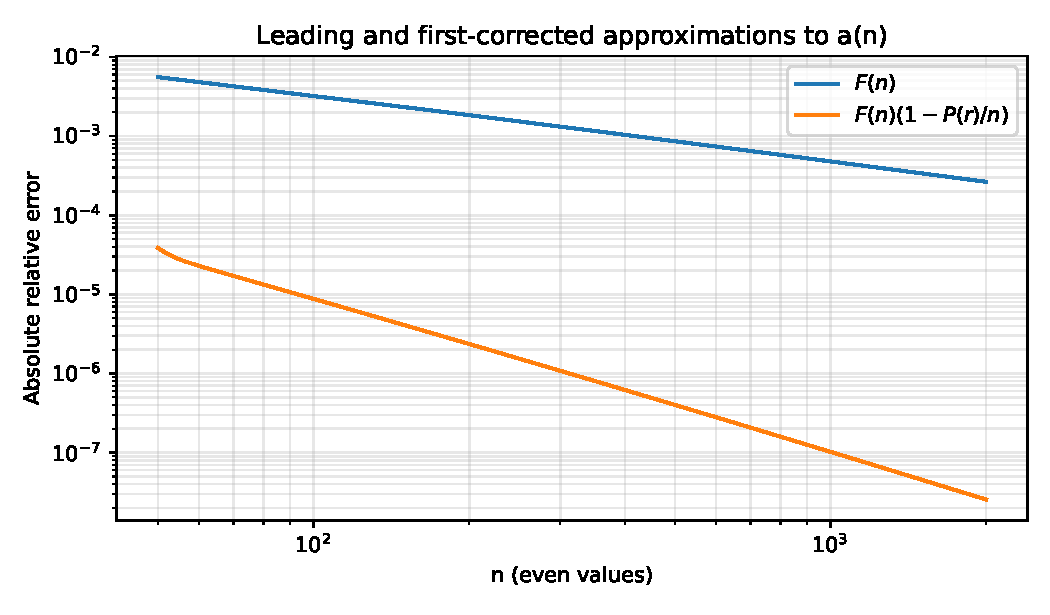
\includegraphics[width=.88\linewidth]{figures/bell_accuracy.pdf}
\caption{Absolute relative errors against exact $a(n)$ for even
$n\ge50$. The first correction improves the approximation by several
orders of magnitude over the plotted range. These are numerical
observations; the proved error orders are in Theorem~\ref{thm:main}.}
\label{fig:bell}
\end{figure}

\begin{table}[htbp]
\centering\small
\begin{tabular}{r r r r}
\toprule
$n$ & $n(D_n/S(n,K_n)-1)$ & $T(n)/D_n-1$ & $T_1(n)/D_n-1$ \\
\midrule
50 & $6.8039771$ & $-3.8391\times10^{-2}$ & $2.5621\times10^{-2}$ \\
51 & $7.4749692$ & $-1.0536\times10^{-1}$ & $9.1698\times10^{-3}$ \\
100 & $7.3721086$ & $-2.6107\times10^{-2}$ & $6.3077\times10^{-3}$ \\
101 & $7.7167024$ & $-5.889\times10^{-2}$ & $1.9435\times10^{-3}$ \\
400 & $7.7380382$ & $-7.8721\times10^{-3}$ & $3.8331\times10^{-4}$ \\
401 & $7.8241196$ & $-1.5923\times10^{-2}$ & $9.8749\times10^{-5}$ \\
2000 & $7.8228653$ & $-1.6463\times10^{-3}$ & $1.5175\times10^{-5}$ \\
2001 & $7.8400188$ & $-3.2484\times10^{-3}$ & $3.6707\times10^{-6}$ \\
\bottomrule
\end{tabular}

\caption{The endpoint ratio and the two parity-sensitive tail
approximations. The second column tends to
$\rho=7.8431072691\ldots$.}
\label{tab:tail}
\end{table}

Table~\ref{tab:tail} confirms the different parity corrections. These are
asymptotic formulas: adding a term need not improve small-$n$ accuracy.
The diagnostics file includes small values as well as large ones.

\begin{figure}[htbp]
\centering
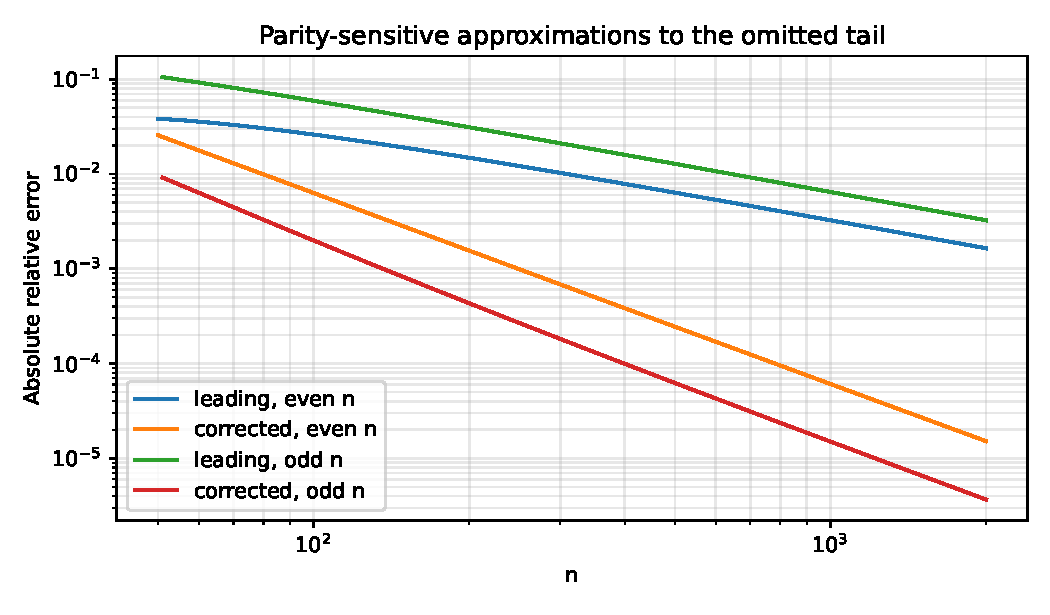
\includegraphics[width=.88\linewidth]{figures/tail_accuracy.pdf}
\caption{Relative tail errors for the leading and first-corrected
formulas, shown separately for even and odd indices. The exact tail is
computed as a sum of Stirling numbers, avoiding cancellation.}
\label{fig:tail}
\end{figure}

\begin{figure}[htbp]
\centering
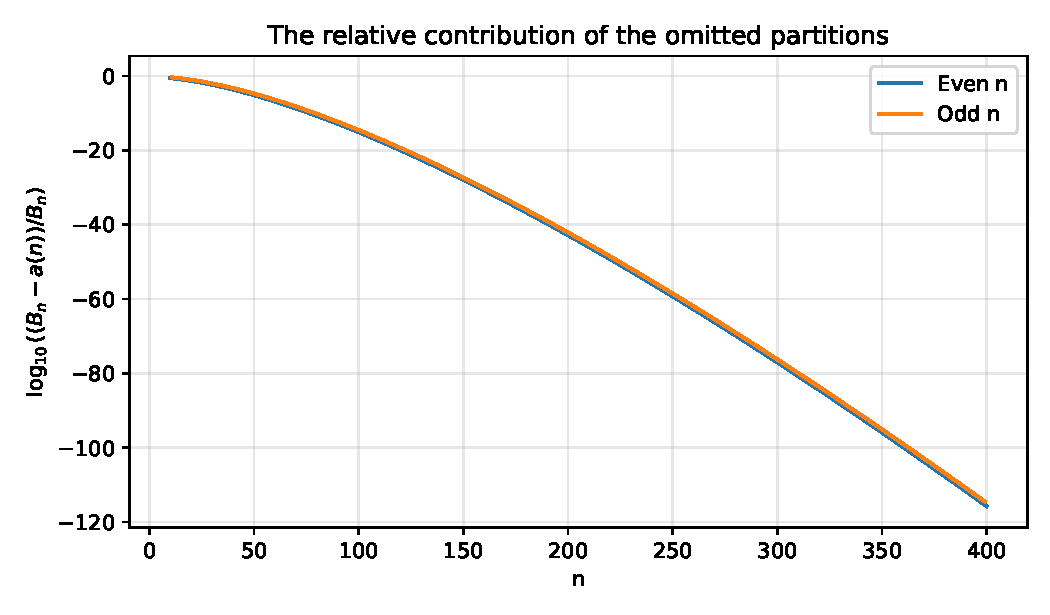
\includegraphics[width=.88\linewidth]{figures/relative_deficit.pdf}
\caption{The base-10 logarithm of the omitted proportion. The small
parity effect is visible, but does not alter the leading Bell growth.}
\label{fig:deficit}
\end{figure}

\subsection{Stable evaluation}
For a large index, evaluate the logarithm first:
\begin{equation}\label{eq:eval}
 \log F(n)=n(r-1+r^{-1})-1-\tfrac12\log(1+r),\qquad r=W_0(n).
\end{equation}
Exponentiate only when a numerical value rather than its logarithm is
needed. For the deficit, use $\log T(n)-\log F(n)$, or compute $D_n/B_n$
from separate exact integers. Computing $1-a(n)/B_n$ in fixed precision
will eventually return zero even though $D_n>0$.

The supplied script uses 80-decimal-digit arithmetic for approximations.
Its exact integer counts are unaffected by that precision setting.
The tail probability can have an exponent below $-400$ or $-900$ without
requiring 400 or 900 mantissa digits, because it is evaluated directly,
not obtained by subtracting a number close to one.

\subsection{Archive contents and commands}
The archive includes this source and compiled PDF, the Python programs,
three figures in PDF and PNG formats, an independently generated exact
table for $0\le n\le1000$, a diagnostic CSV for $2\le n\le2001$, and a
machine-readable verification summary. An OEIS-style formula note is
included as a convenient extract; no submission to OEIS has been made.

The mathematical proofs do not depend on external software, a network
connection, or any unverified numerical hypothesis. From the archive
directory, the calculations and article can be rebuilt with
\begin{lstlisting}
python -m pip install -r requirements.txt
python code/analyze.py --max-n 2001 --plots
python code/make_tables.py
latexmk -pdf -interaction=nonstopmode A277364_asymptotics.tex
\end{lstlisting}

\FloatBarrier
\section{Conclusion}
The requested growth rate is fully determined by the classical Bell
saddle. The cutoff at $n/2$ is asymptotically far enough to the right that
it does not change any fixed algebraic-order relative expansion. The
precise leading equivalent is~\eqref{eq:equivalent}, and its first
correction is~\eqref{eq:main}.

The restriction nevertheless has a sharply describable signature on its
own scale. The difference $B_n-a(n)$ is controlled by the first omitted
Stirling number, with an explicit correction for the rest of the tail.
It grows like $(C\sqrt n)^n$ with a parity-dependent power of $n$, whereas
$B_n$ grows on the much larger $(n/\log n)^n$ scale. Equations
\eqref{eq:tailfirst} and~\eqref{eq:deficitfirst} quantify both effects.
These are sequence-specific applications and refinements of classical
coefficient asymptotics, not claims of a new general Bell-number theory.

\begin{thebibliography}{9}

\bibitem{oeis}
The OEIS Foundation Inc.,
\emph{A277364: Number of ways to partition a set of $n$ elements into at
most $n/2$ disjoint subsets}.
Contributed by Vladimir Reshetnikov, 10 October 2016; retrieved entry
revision dated 16 July 2025.
\url{https://oeis.org/search?q=id:A277364&fmt=text}.
Accessed 20 September 2026.

\bibitem{oeis-bfile}
Indranil Ghosh,
\emph{Table of $n$, A277364$(n)$ for $n=0,\ldots,400$}.
Linked from the OEIS entry.
\url{https://oeis.org/A277364/b277364.txt}.
Accessed 20 September 2026.

\bibitem{dlmf-bell}
NIST Digital Library of Mathematical Functions,
\emph{\S26.7: Set Partitions: Bell Numbers}, particularly
(26.7.2), (26.7.5)--(26.7.8).
\url{https://dlmf.nist.gov/26.7}.
Accessed 20 September 2026.

\bibitem{dlmf-stirling}
NIST Digital Library of Mathematical Functions,
\emph{\S26.8: Set Partitions: Stirling Numbers}.
\url{https://dlmf.nist.gov/26.8}.
Accessed 20 September 2026.

\bibitem{dlmf-w}
NIST Digital Library of Mathematical Functions,
\emph{\S4.13: Lambert $W$-Function}, particularly (4.13.4) and (4.13.10).
\url{https://dlmf.nist.gov/4.13}.
Accessed 20 September 2026.

\bibitem{moser-wyman}
L. Moser and M. Wyman,
\emph{An asymptotic formula for the Bell numbers},
Transactions of the Royal Society of Canada, Series III, Section III,
\textbf{49} (1955), 49--53; accompanying table on p.~54.
Scanned original:
\url{https://oeis.org/A000110/a000110_4.pdf}.
Accessed 20 September 2026.

\end{thebibliography}
\end{document}
